% !TeX root = ../Book5.tex
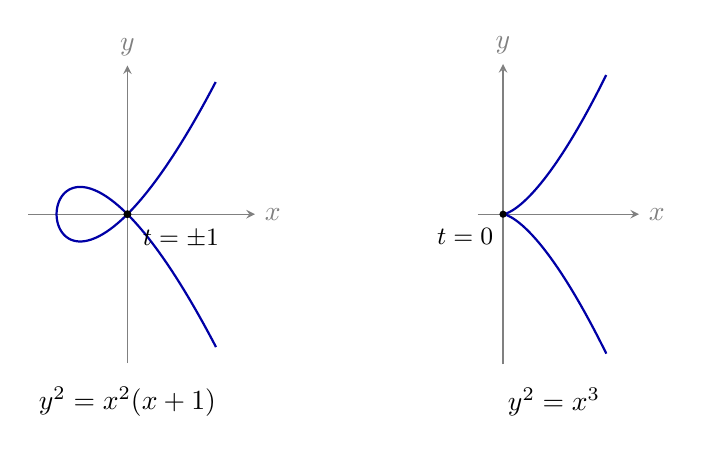
\begin{tikzpicture}[>=stealth,scale=.9]
	\begin{scope}[xshift=0cm]
		\draw[->,gray] (-1.4,0)--(1.8,0) node[right]{\(x\)};
		\draw[->,gray] (0,-2.1)--(0,2.1) node[above]{\(y\)};
		\draw[thick,blue!65!black,domain=-1.5:1.5,samples=151,variable=\t]
			plot ({\t*\t-1},{\t*(\t*\t-1)});
		\fill (0,0) circle (1.6pt);
		\node[below right,font=\small] at (.08,-.08){\(t=\pm1\)};
		\node at (0,-2.65){\(y^2=x^2(x+1)\)};
	\end{scope}
	\begin{scope}[xshift=5.3cm,scale=.8]
		\draw[->,gray] (-.45,0)--(2.4,0) node[right]{\(x\)};
		\draw[->,gray] (0,-2.65)--(0,2.65) node[above]{\(y\)};
		\draw[thick,blue!65!black,domain=-1.35:1.35,samples=121,variable=\t]
			plot ({\t*\t},{\t*\t*\t});
		\fill (0,0) circle (1.8pt);
		\node[below left,font=\small] at (0,-.08){\(t=0\)};
		\node at (.9,-3.31){\(y^2=x^3\)};
	\end{scope}
\end{tikzpicture}
